\documentclass[12pt,twoside]{article}
\renewcommand{\rmdefault}{cmr}
\renewcommand{\sfdefault}{cmss}
\renewcommand{\ttdefault}{cmtt}
\usepackage[T1]{fontenc}
\usepackage[utf8]{inputenc}
\usepackage[english,spanish,es-tabla]{babel}
\usepackage[letterpaper]{geometry}
\usepackage{xltxtra}
\setmainfont[Mapping=tex-text]{Arial}
\geometry{verbose,nomarginpar,tmargin=3cm,bmargin=3cm,lmargin=3cm,rmargin=3cm}
\setlength{\parskip}{\medskipamount}
\setlength{\parindent}{0pt}
\usepackage{array}
\usepackage{float}
\usepackage{setspace}
\usepackage{graphicx}
\doublespacing
\usepackage{caption}
%% Para importar de Excel a Overleaf
\usepackage{booktabs}
\usepackage{longtable}  
\usepackage[table]{xcolor}
\usepackage{multicol}
 \usepackage{lscape}
\definecolor{gris}{rgb}{.851,.851,.851}
\renewcommand{\arraystretch}{2}
\thispagestyle{empty}
\captionsetup{justification=centering}
\usepackage[unicode=true,
 bookmarks=true,bookmarksnumbered=false,bookmarksopen=false,
 breaklinks=false,pdfborder={0 0 0},backref=section,colorlinks=true, linkcolor=blue]
 {hyperref}
\hypersetup{
    colorlinks=false,
    linkcolor=blue,
    filecolor=magenta,      
    urlcolor=cyan,
}

\makeatletter

%% Los convertidores HTML no saben que es tabularnewline
\providecommand{\tabularnewline}{\\}

% No generar la salida para \date
\date{}
% Utilizar el punto decimal, en vez de la acostumbrada coma del español.
% Esto está de acuerdo con la Norma NTC/ISO 80000-1
\decimalpoint

% Etiqueta de figura y tabla a la izquierda seguida de punto.
\usepackage[justification=justified, singlelinecheck=false, labelsep = period]{caption}
% Centrar títulos de secciones
\usepackage{sectsty}
\thispagestyle{empty}


\raggedbottom
\begin{document}

\begin{titlepage}
\begin{center}


{\Large \textbf{Evaluación del comportamiento de sistemas de almacenamiento por baterías bajo la influencia de fenómenos de calidad de potencia en la red eléctrica.}}\\%la función "Huge" es para aumentar el tamaño de letra considerable, esos dobles backslash ayudan a saltar linea  
\vspace*{2\baselineskip}
\textbf{Autores}\\
\vspace*{0.2\baselineskip}
Edwar Santiago Rodriguez Rodriguez \\[0.2cm]
Daniel Alejandro Moya Diaz\\[0.2cm]

\vspace*{3.5\baselineskip}
Director:\\
Andres Felipe Guerrero\\
\vspace*{2\baselineskip}


\vfill %rellena espacios en blanco por lo que usted escriba
\textbf{Universidad de Cundinamarca} \\
Facultad de Ingeniería\\
Programa de Ingeniería Electrónica\\
Fusagasug\'{a},Colombia\\
2023

\end{center}
\end{titlepage}
\newpage
\begin{center}
{\LARGE \textbf{Información del proyecto de investigación }}
\end{center}
\vspace*{0.09\baselineskip}
\hrule
\vspace*{0.2\baselineskip}
\vspace*{0.05\baselineskip}
\textbf{Titulo:} Desarrollo de Microredes y almacenamiento (ESS) prestadores de
servicios complementarios para incrementar la cobertura, eficiencia y confiabilidad del servicio en el departamento de Cundinamarca.\\
\noindent
\textbf{Convocatoria en el cual fue aprobado:} 18 del 2021 Minciencias\\
\textbf{Programas e instituciones vinculados:} Gobernación de Cundinamarca, ENEL-Codensa, Universidad Nacional de Colombia, Universidad de Cundinamarca.\\
\textbf{Duración:} 4 años\\
\textbf{Grupo de investigación en el cual está inscrito el proyecto:} GIGATT, GITEINCO, Electrical Machines \& Drives.
\newpage
\section{Contexto}
\vspace*{0.08\baselineskip}
\hrule
\vspace*{0.2\baselineskip}
El proyecto de investigación marco tiene como objetivo desarrollar Microrredes (MG) y tecnologías de almacenamiento (ESS) que permitan el uso eficiente de la energía eléctrica  para aumentar la cobertura y confiabilidad del servicio en zonas no interconectadas \cite{microgrid}.

El propósito de las MG es integrar fuentes de energía convencionales y no convencionales para contribuir en la mejora de la calidad de servicio en donde la continuidad se ve afectada por las fallas de la red de distribución. Por otra parte, la mitigación de gases de efecto invernadero es de suma importancia para el desarrollo sostenible medioambiental en donde la incorporación de tecnologías energéticas sostenibles son relevantes en el desarrollo de las microrredes. Por lo tanto, se realizará una implementación  piloto de MG basado en sistemas de generación diésel y ESS integrado a una plataforma de red inteligente para el control, monitoreo y supervisión del sistema con el objetivo de identificar la relación óptima de capacidad entre la generación con recursos energéticos distribuidos, plantas Diésel y ESS   \cite{microgrid}.

La implementacion de la microrred busca prestar servicios complementarios para incrementar la cobertura, eficiencia energética y confiabilidad del servicio en el departamento de Cundinamarca \cite{microgrid}. Para ello, el proyecto marco se desarrollará en las siguientes fases (Figura 1):
\newpage
\begin{figure}[h!]
    \begin{center}
    \centering
    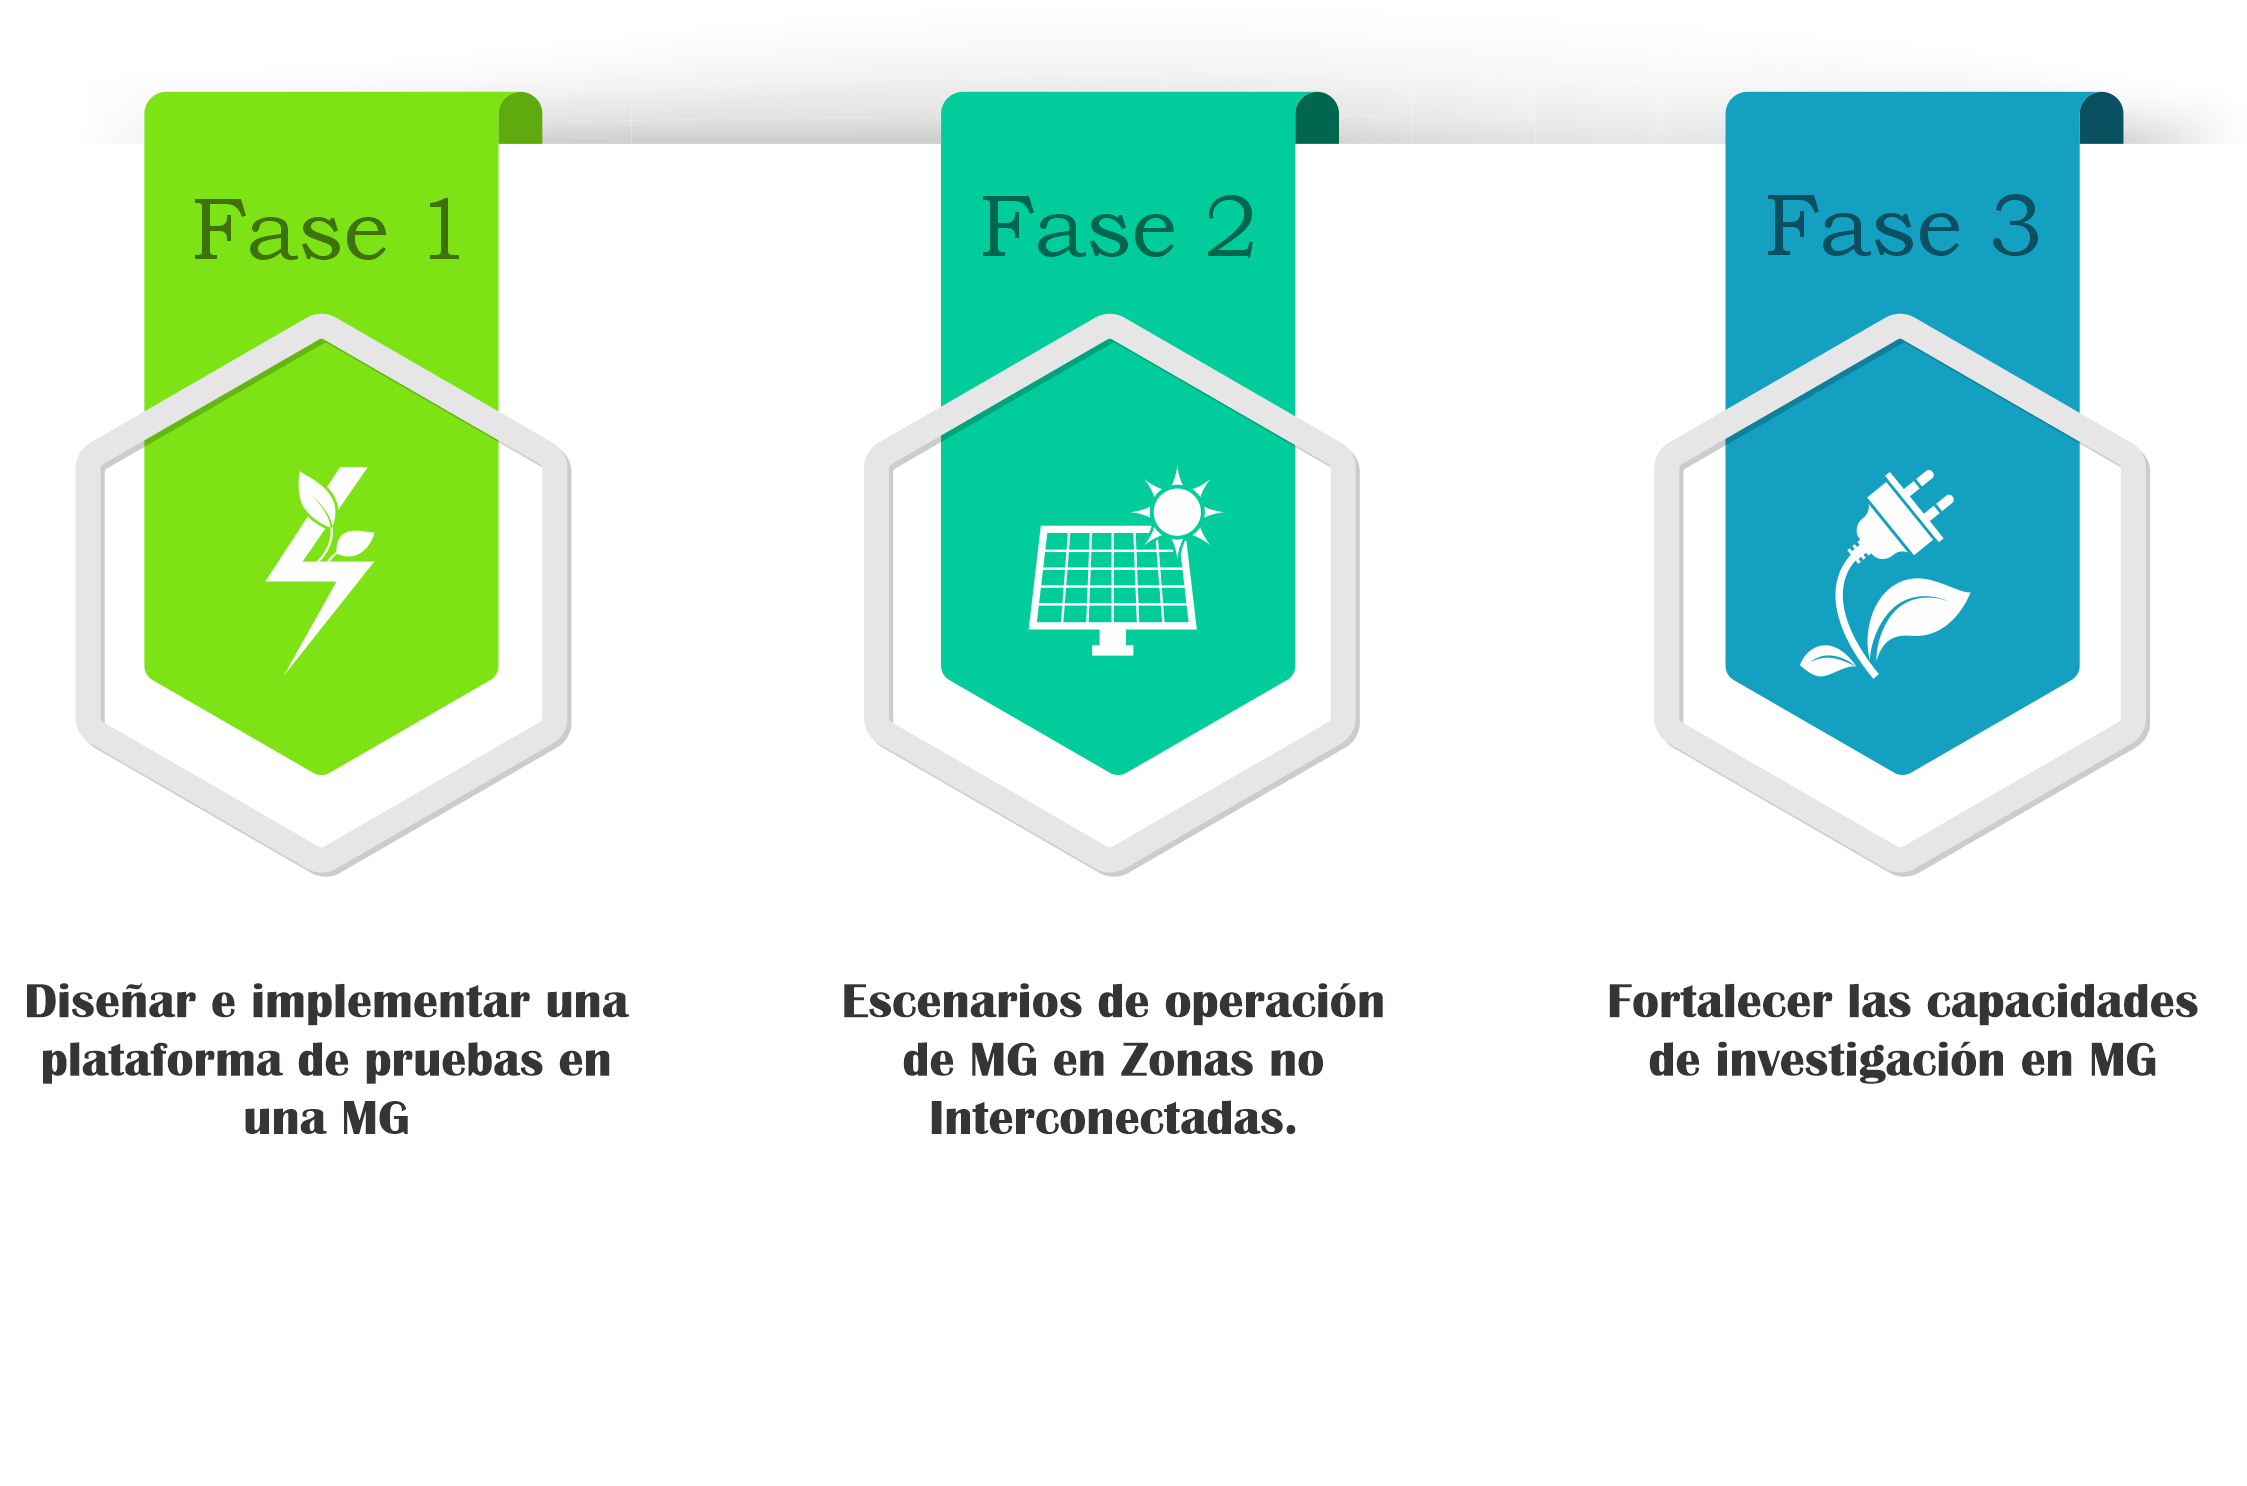
\includegraphics[scale=0.75]{Imágenes/contexto/Fases.png}
	\caption{ Fases proyecto marco}
    \end{center}
\end{figure}

\textbf{Fase 1: } Consulta de revistas especializadas, normas y artículos con el objeto de realizar pruebas enfocadas en las variables más relevantes que monitorean la MG para realizar una adquisición de datos que logre determinar los puntos óptimos de operación de la microrred.\\

\textbf{Fase 2: } Desarrollo de  modelos en simulación que permita establecer el comportamiento de la MG en diferentes escenarios, con el fin de desarrollar  artículos de investigación que permitan la presentación de los resultados obtenidos del proyecto.\\

\textbf{Fase 3: } Realizar capacitaciones acerca de las MG para garantizar su funcionamiento,  elaborando manuales de operación referente a la investigación, con la finalidad de ejecutar el proyecto de manera eficiente.


El trabajo de grado aportará al proyecto marco en la fase 2 mediante la investigación acerca del comportamiento en tecnologías de baterías existentes en el mercado considerando la  interacción con la red eléctrica bajo fénomenos de calidad de potencia. La investigación se realizará a través de revisión bibliográfica en fuentes verídicas tales como revistas indexadas, trabajos de grado, artículos científicos e información de instituciones vinculadas al proyecto para posteriormente establecer escenarios de pruebas mediante simulación.

\newpage
\section{Antecedentes}
\vspace*{0.08\baselineskip}
\hrule
\vspace*{0.7\baselineskip}
Los Sistemas de Almacenamiento por Baterías  ( BESS por sus siglas en inglés ) mediante el uso de  energías renovables y no convencionales son de suma importancia  para la mitigación de problemas en el suministro de energía eléctrica; a partir de las necesidades requeridas se debe realizar un diagnóstico tecnológico que permita clasificar y seleccionar  diferentes tipos de baterías adecuadas. Alrededor del mundo, se han desarrollado diferentes proyectos que se basan en los Sistemas de Almacenamiento por Baterias, entre los cuales cabe destacar:

Japón incrementó el porcentaje de nuevas energías como solar, eólica y biomasa a un 3\%; en Rokkasho se instaló un parque eólico de 51 MW de potencia nominal y un parque de baterías de Sulfuro de Sodio (NAS) con capacidad de  34 MW para mitigar las fluctuaciones generadas por energías renovables \cite{parques_eolicos}. En la Figura 2, existe una relación de los ciclos  carga/descarga de la batería evidenciando que esta compensa las fluctuaciones de la potencia eólica suministrada en un ciclo de descarga y vuelve a un estado de carga cuando la energía eólica puede mantener un nivel óptimo de potencia.
\begin{figure}[h!] %%BATERIASSECCIONES
    \begin{center}
    \centering
    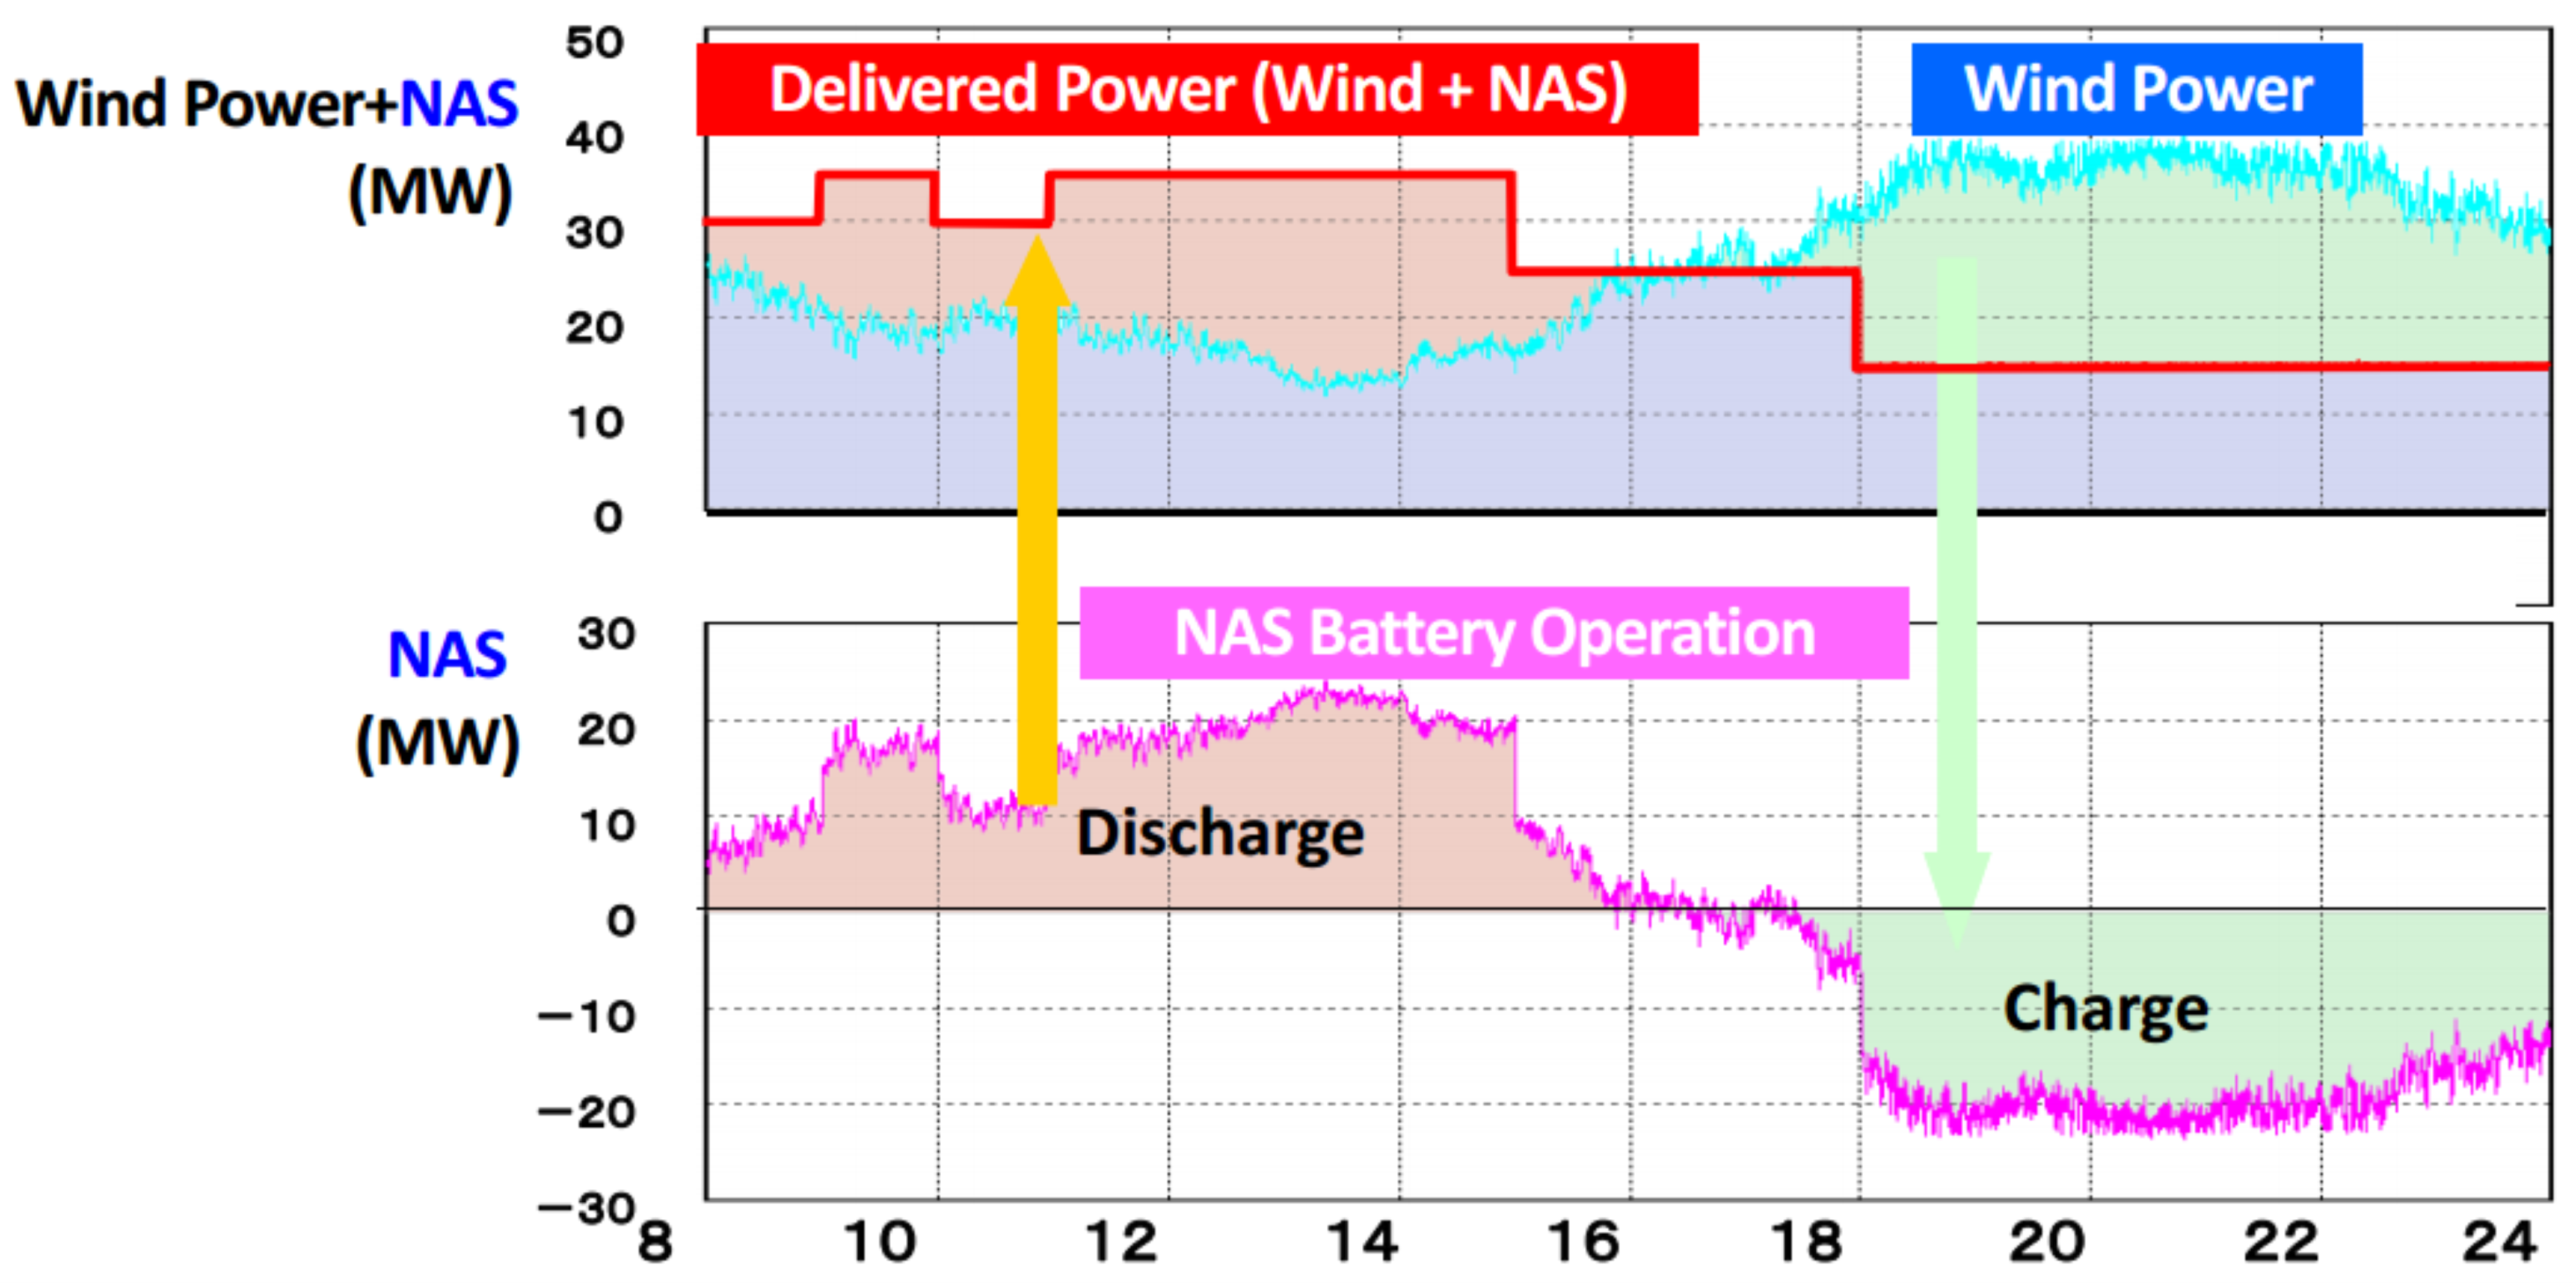
\includegraphics[scale=0.3]{Imágenes/Estado del arte/nas+wind.png}
	\caption{ Curva de generación de energía eléctrica parque eólico Rokkasho \cite{bess_zarate}}
    \end{center}
\end{figure}
\newpage
M5BAT es un sistema BESS híbrido para brindar reserva de contención de frecuencia (FCR) con potencia total de 5 MW en Alemania. El sistema está compuesto por bancos de baterías de plomo-ácido y ión-litio con una capacidad total de 5,8 MWh. \cite{BESS_GERMANY}. En la Figura 3, se realiza una comparación de potencia FCR y energía acumulada en un día así como el promedio de 12 horas en el año. El objetivo es obtener numerosas acciones de gestión energética para mejorar la comparabilidad entre el promedio de potencia y el rendimiento de energía; los resultados de laboratorio entregan una mayor potencia en promedio y un mayor rendimiento en el perfil de 12 horas debido al cambio del estado de carga de la batería durante todo el día.
\begin{figure}[h!]
    \begin{center}
    \centering
    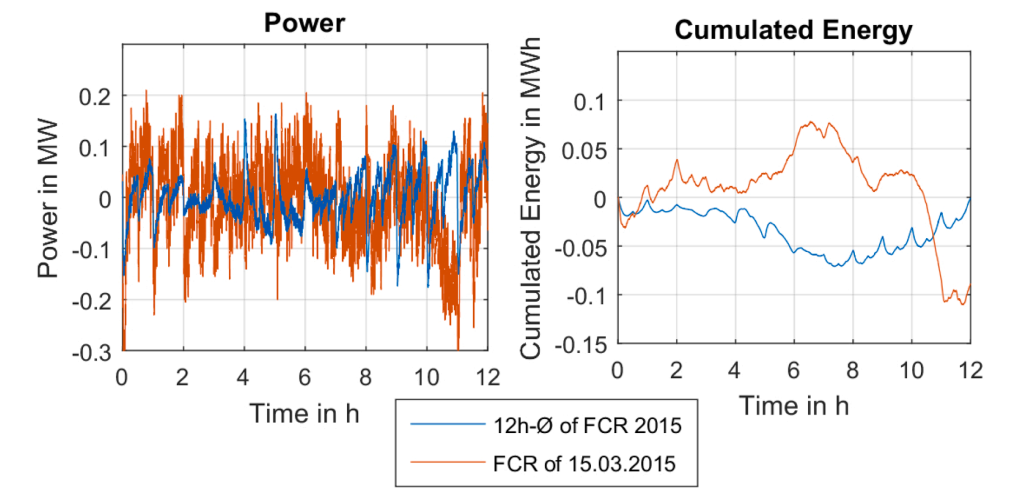
\includegraphics[scale=0.62]{Imágenes/Estado del arte/FCR ACIDO.png}
	\caption{ Comparación de potencia FCR en el año 2015 \cite{BESS_GERMANY}}
    \end{center}
\end{figure}
\newline
Los edificios consumen el 29\% de la energía en Japón; por lo tanto, para dar un aprovechamiento de la energía solar se implementó un esquema de control de potencia eficiente y un sistema independiente híbrido renovable que proporcione una salida con baja distorsión armónica. El sistema es instalado en el techo de los edificios de la ciudad de Kasuga, consiste de tres módulos de paneles solares con una potencia total de 480 W, una turbina de viento de 400 W y una batería de plomo ácido con una capacidad de 30 Ah \cite{BESS_KASUGA_JAPON}.

En la Figura 4, se visualiza la potencia promedio de salida en las fuentes de energía y la potencia consumida por la carga; el sistema de control extrae la máxima potencia del PV, la turbina y la batería en respuesta a los requerimientos de la carga. Por lo tanto, en el momento que exista un cambio en el entorno o dinámica del sistema, el sistema de control balancea el flujo de potencia de forma inmediata. 
\begin{figure}[h!]
    \begin{center}
    \centering
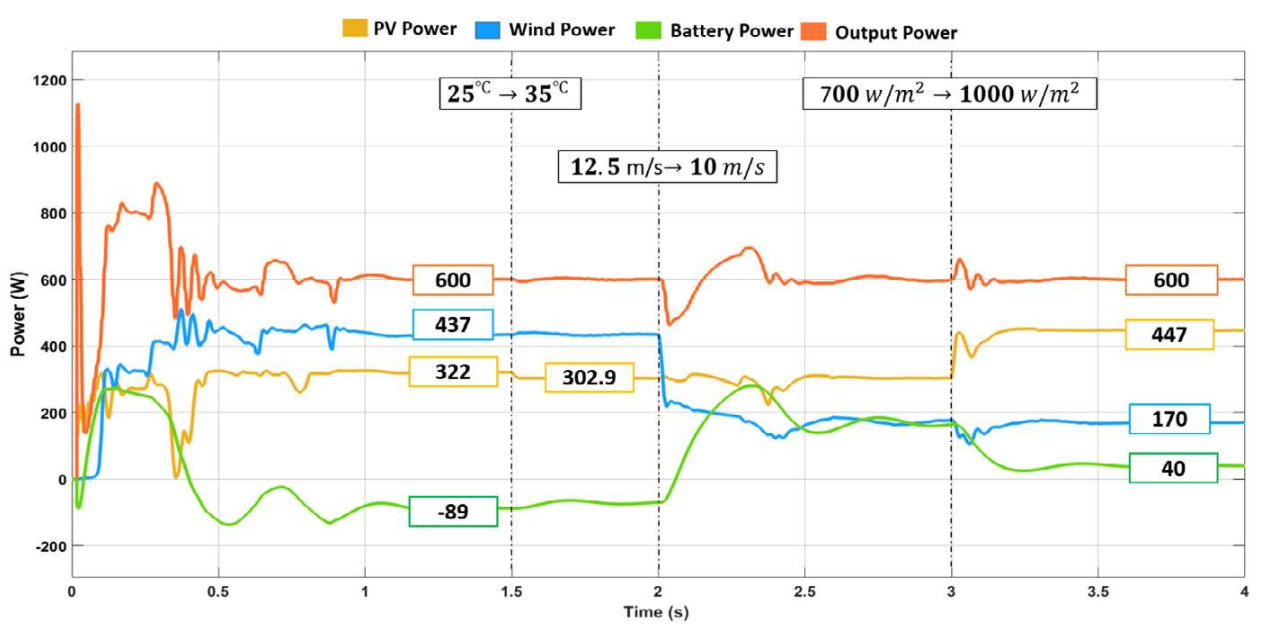
\includegraphics[scale=0.6]{Imágenes/Estado del arte/besskasuga.png}
	\caption{ Características de descarga de la batería \cite{BESS_KASUGA_JAPON}}
    \end{center}
\end{figure}

En el norte de China se implementó un proyecto para  la co-optimización de  la capacidad del sistema de almacenamiento de energía térmica y de baterías en sistema complementario de energía múltiple con plantas eólicas (300 MW), estaciones fotovoltaícas (300 MW), planta de energía termosolar (50 MW) y una batería de Ión Litio (50 MW); el sistema tiene como objetivo maximizar la utilidad anual de las energías renovables \cite{li2019capacity}.

En la Figura 5 , se visualiza la salida de cada sistema multi energía en tres días; la batería se carga durante el día cuando el suministro de energía es  proporcionado mayoritariamente por las fuentes fotovoltaícas y eólicas. De la misma forma, la descarga de la batería sucede en la noche suministrando energía eléctrica  junto con la fuente de energía solar concentrada (CSP).
\begin{figure}[h!]
    \begin{center}
    \centering
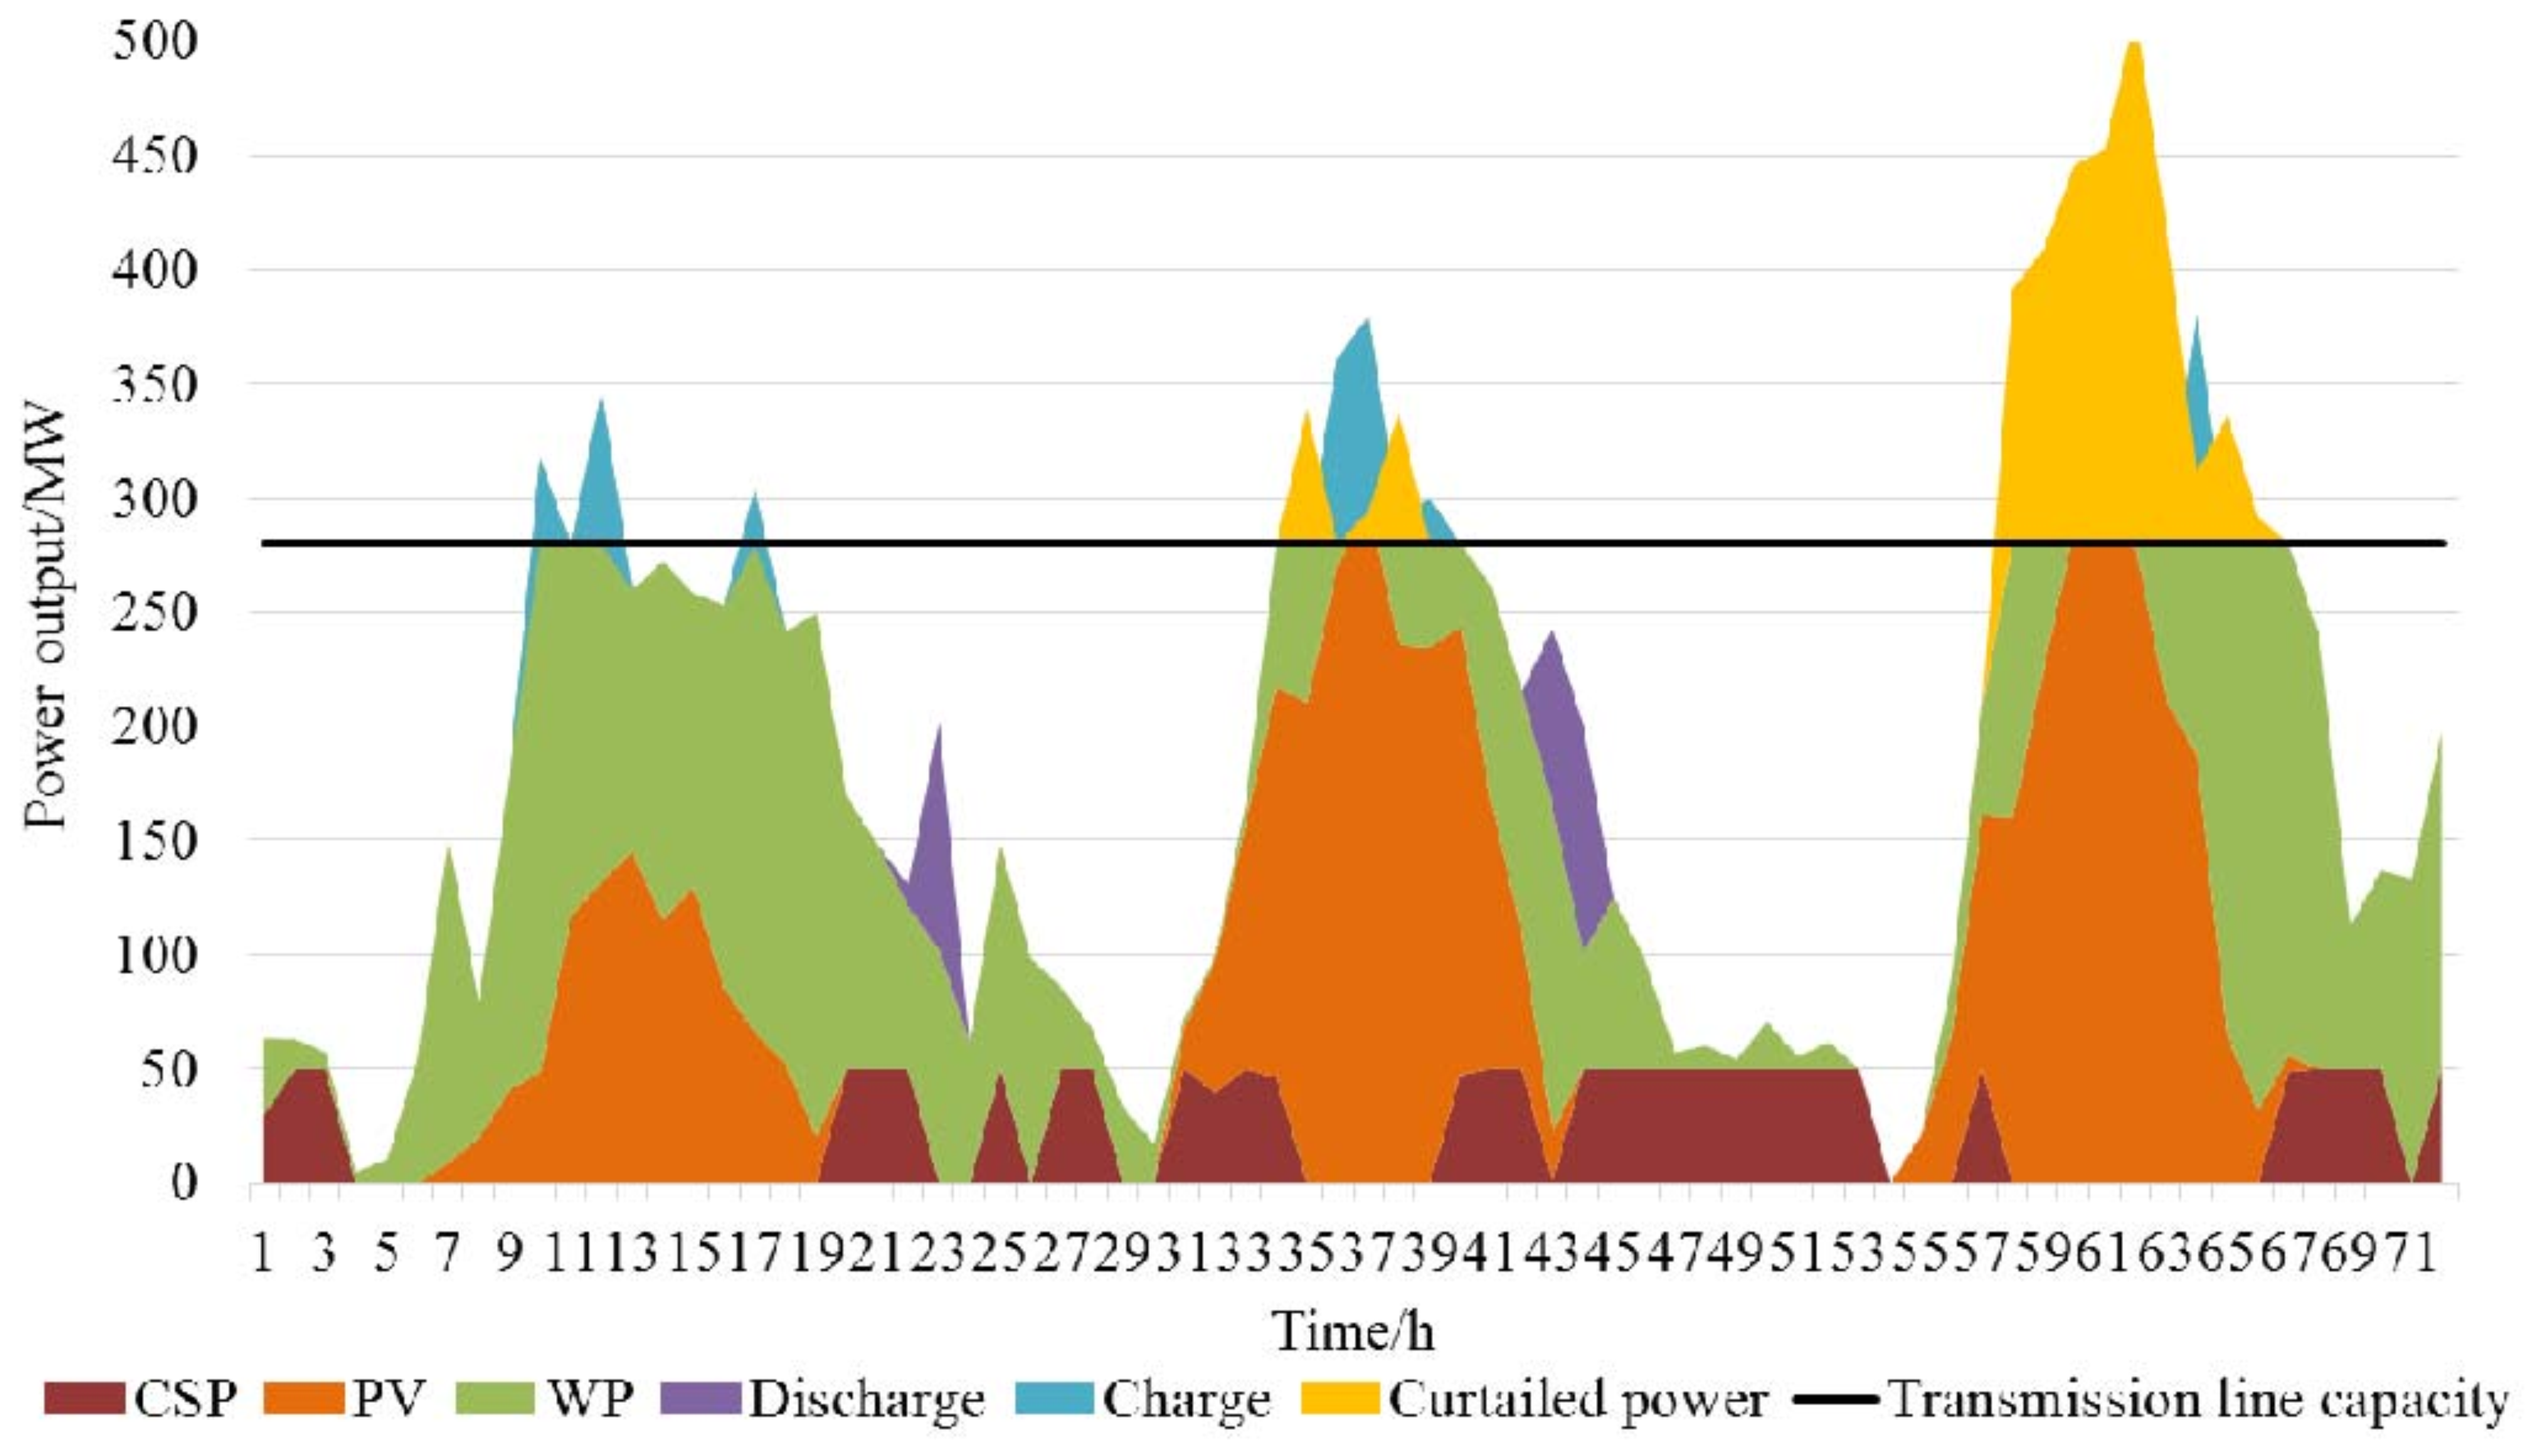
\includegraphics[scale=0.4]{Imágenes/Estado del arte/Energiatermica.png}
	\caption{Salida de potencia sistema multi energía
	\cite{li2019capacity}}
    \end{center}
\end{figure}
\newline
En Medellín-Colombia se realizó una investigación sobre la evaluación del desempeño de microrredes aisladas en áreas no interconectadas donde se analiza la integración de energía generada mediante fuentes diesel y fotovoltaicas integradas con sistemas BESS. En la figura 6 , se evidencia la media horaria de todo el año correspondiente a la energía utilizada para cargar el sistema BESS, donde el modelo prioriza la fuente fotovoltaica debido a sus bajos costos y solo se utiliza el generador diesel cuando la fuente fotovoltaica no produce la energía necesaria para caragar el sistema BESS \cite{ropero2022sizing}.
\newpage
\begin{figure}[h!]
    \begin{center}
    \centering
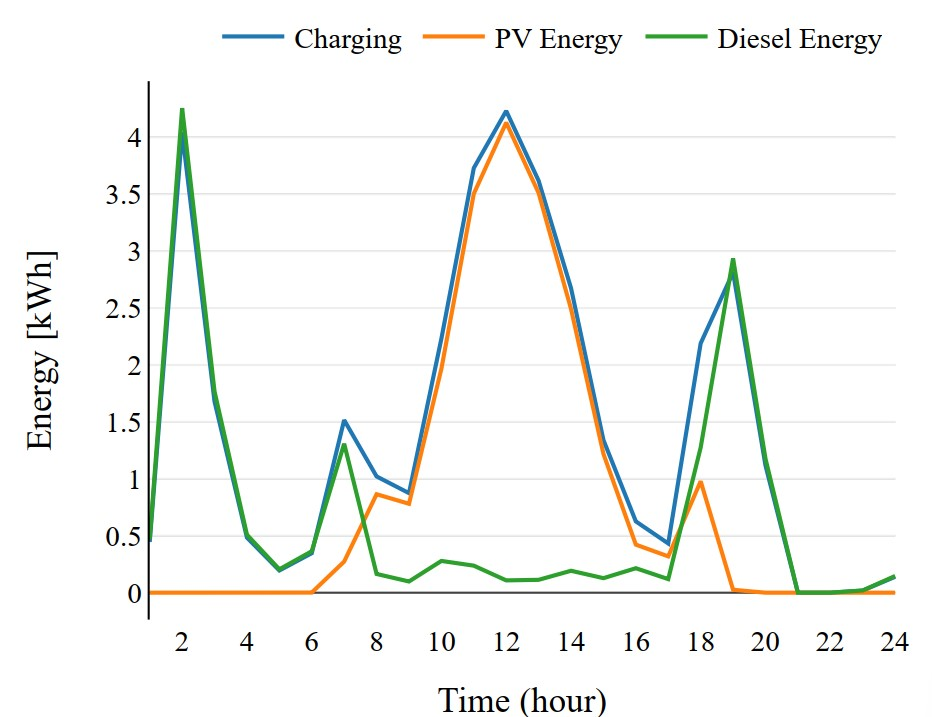
\includegraphics[scale=0.58]{Imágenes/Estado del arte/BESS-PV-DG.jpg}
	\caption{Promedio de energía para cargar el sistema BESS \cite{ropero2022sizing}.}
    \end{center}
\end{figure}

\smallskip






\newpage
\section{Objetivos}
\vspace*{0.08\baselineskip}
\hrule
\vspace*{0.7\baselineskip}
\subsection{Objetivo general}
Evaluar el comportamiento de tecnologías de baterías en sistemas de almacenamiento (BESS) considerando la interacción con la red eléctrica bajo la influencia de fenómenos de calidad de potencia.
\subsection{Objetivos específicos}

\begin{itemize}
    \item Realizar una revisión bibliográfica que permita contrastar resultados teóricos y experimentales reportados en la evaluación del comportamiento de sistemas de almacenamiento por baterías en interacción con la red eléctrica
    \item Establecer escenarios de pruebas de sistemas de almacenamiento por baterías a partir de la identificación de fenómenos en la calidad de potencia de la red eléctrica.
    \item Seleccionar a partir de pruebas de simulación, una topología de sistema de almacenamiento por baterías que contribuya en la reducción de problemas de calidad de la potencia en la red.
    
\end{itemize}



\newpage
\section{Metodología}
\vspace*{0.2\baselineskip}
\hrule
\vspace*{0.7\baselineskip}
Para dar cumplimiento a los objetivos planteados en el proyecto , se establecen  las siguientes fases  (Figura 7):

\begin{figure}[h!]
    \begin{center}
    \centering
    \includegraphics[scale=0.7]{Imágenes/Metodología/Fases proyecto BESS.eps}
	\caption{Fases proyecto BESS}
    \end{center}
\end{figure}



\begin{itemize}
    \item 
    \textbf{Fase 1 :} Se indaga acerca del comportamiento  de sistemas de almacenamiento por baterías bajo la influencia de la red eléctrica 
    para realizar una comparación y selección de tecnologías de baterías existentes en el mercado, teniendo en cuenta factores tales como la eficiencia, densidad de energía y ciclo de vida.
    \item 
   \textbf{Fase 2 : }Se establecen escenarios de prueba a través de diferentes topologías simuladas de sistemas de almacenamiento integrando modelos de baterías considerando los fenómenos de calidad de potencia de la red eléctrica que se presentan en la zona de estudio. Posteriormente , se procede a realizar cambios en los escenarios de prueba mediante modificaciones en las topologías con la finalidad de evaluar el comportamiento y desempeño de la batería frente a una alteración en la red eléctrica.
\newpage    
    \item 
    \textbf{Fase 3 : }
    Se realizan pruebas técnicas simuladas en baterías para supervisar parámetros como SOC (estado de carga), densidad de potencia, profundidad de descarga, eficiencia roundtrip y otros procesos relacionados con el objetivo de establecer las mejores condiciones de funcionamiento para la topología del sistema de almacenamiento por baterías, teniendo en cuenta tecnologías de conversión de potencia, calidad de potencia y especificaciones técnicas.
\end{itemize}


\newpage


\section{Marco conceptual}
\vspace*{0.2\baselineskip}
\hrule
\vspace*{0.7\baselineskip}
\subsection{Conceptos claves}
\begin{itemize}
    \item \textbf{Microrred:} cluster de generación distribuida , fuentes locales y cargas que permiten conectarse mediante una red eléctrica en la que se gestiona integralmente la generación, el almacenamiento de energía y las necesidades de las cargas de los usos finales \cite{microgrid}.
    \item \textbf{Sistemas de Almacenamiento de Energía por Baterías (BESS)}: sistema recargable de baterías capaz de almacenar energía de diferentes fuentes y descargarse cuando se necesite. BESS consta de una o más baterías y se puede utilizar para equilibrar la red eléctrica, proporcionar energía de respaldo y mejorar la estabilidad de la red \cite{siemens}.
    \item  \textbf{Estado de Carga (SoC):} medida relativa de la cantidad de energía almacenada en una batería, definida como la relación entre la cantidad de carga extraíble de la celda en un momento específico del tiempo y la capacidad total.
    \item \textbf{Inversor DC-AC:} su función es transformar una tensión de entrada continua a una tensión de salida alterna con una magnitud y frecuencia deseada \cite{rashid-inversor}. El proceso de conmutación se realiza generalmente con transistores MOSFET e IGBT mediante señales PWM con el objetivo de obtener a la salida una señal sinusoidal.
    \item \textbf{Densidad de energía:} cantidad de energía que se puede almacenar en un solo sistema por unidad de volumen o por unidad de peso \cite{densidad}.
\end{itemize}

\newpage
La producción de energía eléctrica es una necesidad del mundo moderno del cual el ser humano no puede prescindir. Por lo tanto, los sistemas de energía eléctrica deben tener la capacidad de suministrar energía suficiente para la cantidad demandada teniendo en cuenta la calidad del servicio, las condiciones ambientales y los costos. Debido a que existe variabilidad en la producción de energías tanto  convencionales y no convencionales, se requiere almacenar energía para maximizar su aprovechamiento. 


\subsection{Tipos de almacenamiento en la red}
En la actualidad existen diferentes tipos de tecnologías para almacenamiento de energía (ESS) dependiendo de su uso. Los dispositivos de almacenamiento se pueden clasificar en mecánicos, electroquímicos, químicos, eléctricos y térmicos \cite{Handbook}. En la Figura 8, se pueden visualizar los tipos de ESS.
\begin{figure}[h!]
    \begin{center}
    \centering
    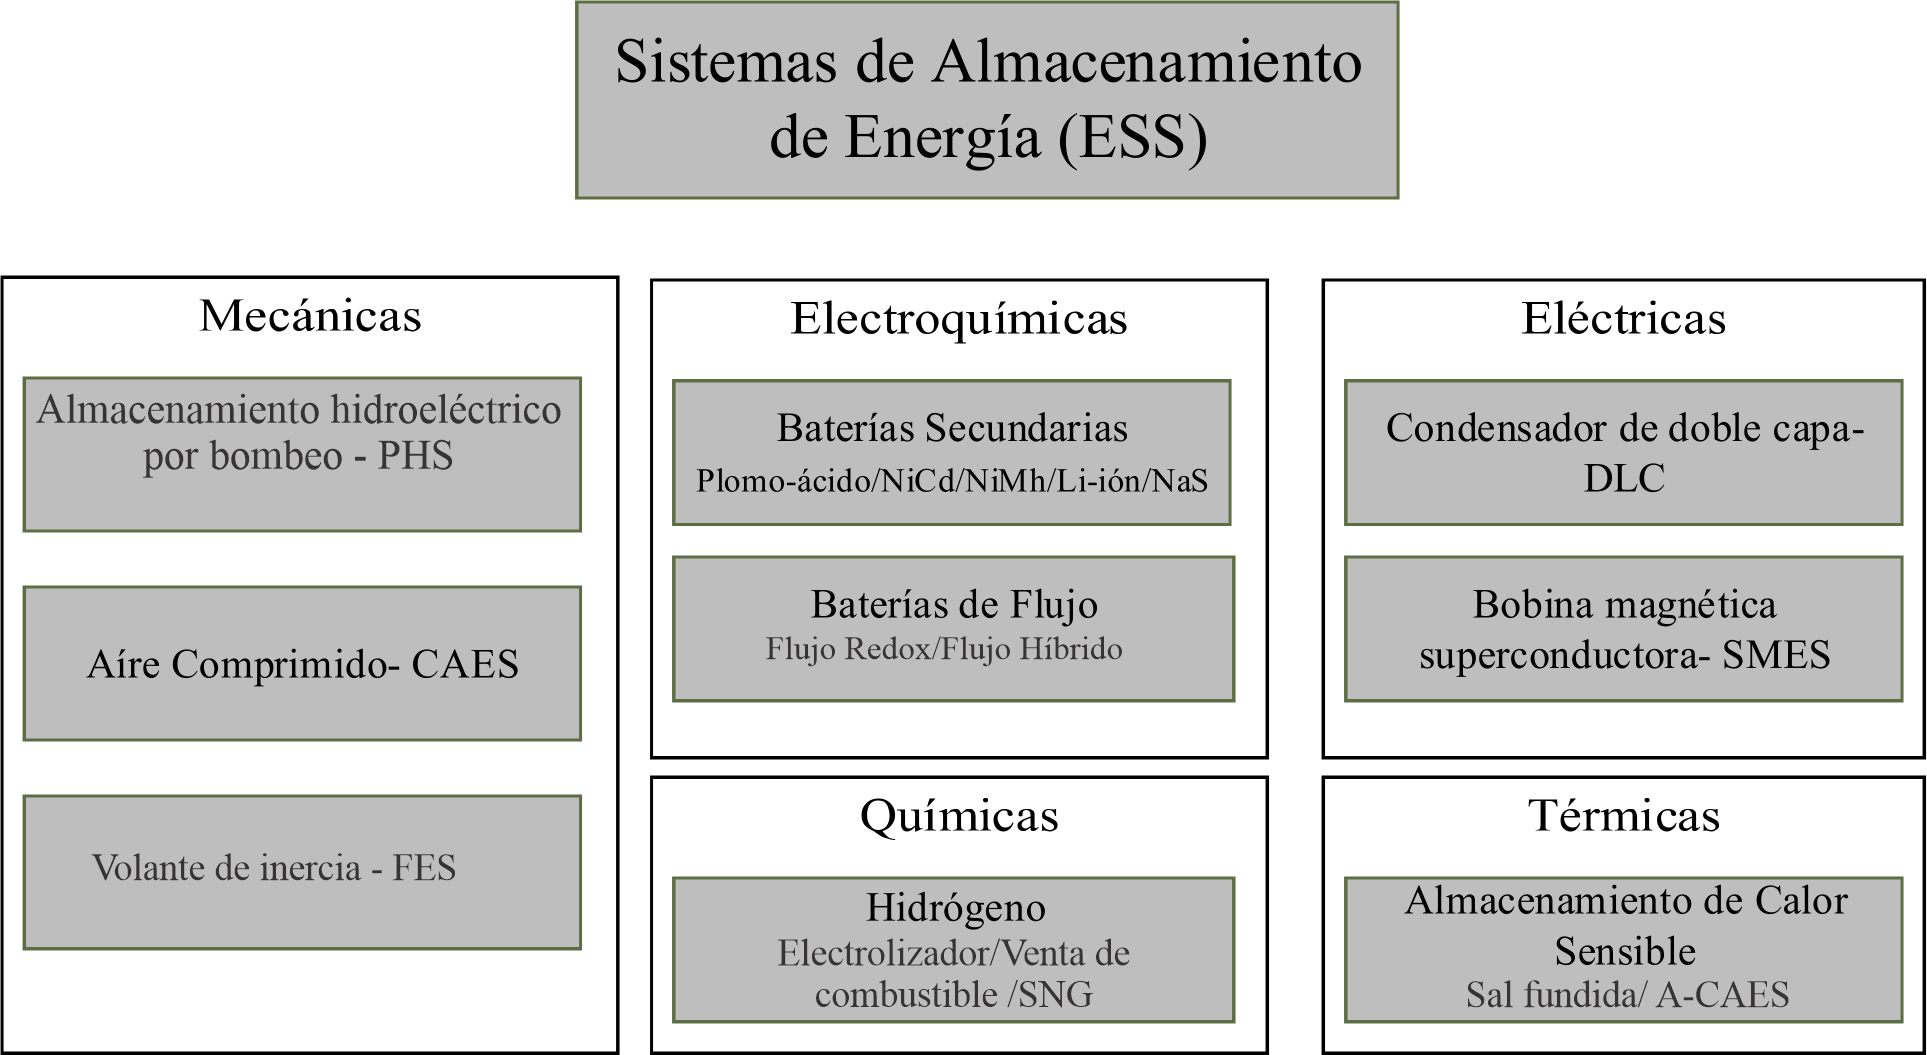
\includegraphics[scale=0.7]{Imágenes/marcoconceptual/Tipos de energias.png}
	\caption{ Clasificación de  los sistemas de almacenamiento de energía (ESS)\cite{bess_distritall}.}
    \end{center}
\end{figure}
\newpage
Los dispositivos de almacenamiento tienen dos fines principales, el suministro de energía ininterrumpida (UPS) o transmisión y soporte del sistema de distribución \cite{Handbook}. En la Tabla 1, se visualiza una comparación más detallada de diferentes tecnologías ESS, clasificándolas por su duración del almacenamiento, número de ciclos o vida útil, autodescarga, densidad de  potencia y tiempo de respuesta.
\begin{table}[htbp]
  \centering
  \caption{Características técnicas de los ESS }
  \resizebox{17cm}{!} {
    \begin{tabular}{|p{13.855em}|c|c|c|c|c|}
    %\toprule
    \rowcolor[rgb]{ .051,  .051,  .051} \multicolumn{1}{|c|}{\textcolor[rgb]{ 1,  1,  1}{\textbf{PARÁMETROS }}} & \multicolumn{1}{p{10.145em}|}{\textcolor[rgb]{ 1,  1,  1}{\textbf{Densidad de potencia (Wkg/kWm)}}} & \multicolumn{1}{p{8.57em}|}{\textcolor[rgb]{ 1,  1,  1}{\textbf{Tiempo de vida (años-ciclos) }}} & \multicolumn{1}{p{8.285em}|}{\textcolor[rgb]{ 1,  1,  1}{\textbf{Tiempo de descarga tipico}}} & \textcolor[rgb]{ 1,  1,  1}{\textbf{Tiempo de recarga }} & \multicolumn{1}{p{8.855em}|}{\textcolor[rgb]{ 1,  1,  1}{\textbf{Auto descarga (\%\textbackslash{}día)}}} \\
    %\midrule
    \rowcolor[rgb]{ .051,  .051,  .051} \multicolumn{1}{|c|}{\textcolor[rgb]{ 1,  1,  1}{\textbf{TECNOLOGÍAS}}} & \textcolor[rgb]{ 1,  1,  1}{} & \textcolor[rgb]{ 1,  1,  1}{} & \textcolor[rgb]{ 1,  1,  1}{} & \textcolor[rgb]{ 1,  1,  1}{} & \textcolor[rgb]{ 1,  1,  1}{} \\
    %\midrule
    \multicolumn{1}{|c|}{Volantes de Inercia} & 400-1600/5000 & >20 (10$^7$) & 15 s-15 min & <15 min & 20-100 \\
    \hline
    \rowcolor{gris} \multicolumn{1}{|c|}{Hidroeléctrica bombeada} & NA/0.1-0.2 & 50-100 (>500) & h-days & 1 min-h & 0 \\
    \hline
    \multicolumn{1}{|c|}{Aire Comprimido} & NA/0.2-0.6 & 25-40  & h-days & min-h & 0 \\
    \hline
    \rowcolor{gris} Supercapacitores/Capacitores de doble capa & 0.1-10/40000-120000 & >20 (5x10$^5$) & ms-1 h & s-min & 2-.40 \\
    \hline
    \multicolumn{1}{|c|}{Batería Ión de litio} & 230-340/1300-10000 & 8-15 (500-6000) & min-h & min-h & 0.1-0.3 \\
    \hline
    \rowcolor{gris} \multicolumn{1}{|c|}{Batería de Cadmio de Níquel} & 150-300/75-700 & 15-20 (2500) & s-h   & 1 h   & 0.2-0.6 \\
    \hline
    \multicolumn{1}{|c|}{Batería Sulfuro de Sodio} & 90-230/120-160 & 12-20 (>2000) & s-h   & 9 h   & 20 \\
    \hline
    \rowcolor{gris} Supercapacitores/Capacitores de doble capa & 0.1-10/40000-120000 & >20 (5x10$^5$) & ms-1 h & s-min & 2-.40 \\
    \hline
    \multicolumn{1}{|c|}{Batería de Ácido de Plomo} & 75-300/90-700 & 3-15 (2000) & min-h & 8-16 h & 0.1-0.3 \\
    \hline
    \rowcolor {gris} \multicolumn{1}{|c|}{Batería de Bromuro de Zinc} & 50-150/1-25 & 5-10 (300-1500) & s-10 h & 4 h   & 0-1 \\
    \hline
    Batería de Reducción-Oxidación de Vanadio & NA/0.5-2 & 10-20 (13x10$^3$) & s-10 h & min   & 0-10 \\
    \bottomrule
    \end{tabular}%
    }
  \label{tab:addlabel}%
\end{table}%
\newline
Los sistemas BESS se consideran tecnologías de tiempo de descarga medio (duración entre varios minutos hasta algunas horas) con tecnologías electroquímicas \cite{bess_distritall}. Las tecnologías de baterías para dispositivos de almacenamiento de energía se pueden diferenciar en función de la densidad de energía, tiempo de carga y descarga, esperanza de vida y el impacto ambiental \cite{Handbook}.
\newpage
\begin{table}[htbp]

  \centering
  \caption{Comparación técnicas de los BESS}
  \resizebox{16cm}{!} {
    \begin{tabular}{|p{10em}|c|c|c|c|c|p{11em}|}
    %\toprule
    \rowcolor[rgb]{ .051,  .051,  .051} \multicolumn{1}{|c|}{\textcolor[rgb]{ 1,  1,  1}{\textbf{PARÁMETROS }}} & \multicolumn{1}{p{10em}|}{\textcolor[rgb]{ 1,  1,  1}{\textbf{Potencia AC nominal}}} & \multicolumn{1}{p{10em}|}{\textcolor[rgb]{ 1,  1,  1}{\textbf{Autodescarga}}} & \multicolumn{1}{p{10em}|}{\textcolor[rgb]{ 1,  1,  1}{\textbf{Profundidad de descarga \%}}} & \multicolumn{1}{p{10em}|}{\textcolor[rgb]{ 1,  1,  1}{\textbf{Eficiencia Roundtrip \newline{}\%}}} & \multicolumn{1}{p{10em}|}{\textcolor[rgb]{ 1,  1,  1}{\textbf{Temperatura óptima de diseño}}} & \textcolor[rgb]{ 1,  1,  1}{\textbf{Aplicación}} \\
    %\midrule
    \rowcolor[rgb]{ .051,  .051,  .051} \multicolumn{1}{|c|}{\textcolor[rgb]{ 1,  1,  1}{\textbf{BATERÍAS}}} & \textcolor[rgb]{ 1,  1,  1}{} & \textcolor[rgb]{ 1,  1,  1}{} & \textcolor[rgb]{ 1,  1,  1}{} & \textcolor[rgb]{ 1,  1,  1}{} & \textcolor[rgb]{ 1,  1,  1}{} & \multicolumn{1}{r|}{\textcolor[rgb]{ 1,  1,  1}{}} \\
    %\midrule
    \multicolumn{1}{|c|}{Ión de Litio} & \multicolumn{1}{|c|}{200-500 kW} & 1-2\% mensual  & 100   & 85-95 & 15°C  & Cámaras,  computadores portátiles y dispositivos móviles  \\
    \hline
    \rowcolor{gris} \multicolumn{1}{|c|}{Sulfuro de Sodio} & 50-400 kW & 0.01\%  mensual  & 100   & 89-92 & 300°C–350°C &  Redes de almacenamiento de energía fijas a gran escala \\
    \hline
    \multicolumn{1}{|c|}{Flujo redox} & 50-330 kW & Baja  & 100   & 85-90 & 5°C–35°C &  Aplicaciones \newline{}estacionarias  \\
    \hline
    \rowcolor{gris} \multicolumn{1}{|c|}{Plomo Ácido} & 250-500 kW & 0.1\% mensual & 50    & 80-85 & 45°C  & Sistema de alimentación ininterrumpida o en sistemas   de energía renovable \\
    \hline
    \multicolumn{1}{|c|}{ Níquel-Cadmio} & 125-600 kW & 15-20\% mensual & 50    & 70-90 & 5°C-25°C & Computadores portátiles, taladros, cámaras de video  y otros dispositivos que requieren una descarga  uniforme. \\
    \hline
    \rowcolor{gris} Níquel-Metalhidruro & 500-2000 W & 30\% mensual & 100   & 66    & -30°C a 70°C &  Vehículos, robótica y en electrónica de consumo.    \\
    \bottomrule
    \end{tabular}%
    }
  \label{tab:addlabel}%
  
\end{table}%







Existen diferentes tipos de tecnologías de baterías en el mercado, en la Tabla 2 se realiza una comparación de características técnicas de diferentes baterías en el mercado, especificando los siguientes parámetros:
\begin{itemize}
    \item Potencia AC nominal: ``potencia máxima empleada por una máquina en uso normal" \cite{proyecto_mg}.
    \item Profundidad de descarga: ``la cantidad de energía que se ha extraído de la batería, expresada en porcentaje" \cite{profundidad_descarga}.
    \item Eficencia Roadtrip: ``tiempo de ida y vuelta (RTT) es la duración en milisegundos que tarda una solicitud de red en ir de un punto de partida a un destino y volver al punto de partida" \cite{tiempo_ida_vuelta}.
\end{itemize}



\newpage
\section{Cronograma}



\begin{table}[h!]
    \begin{center}
    \centering
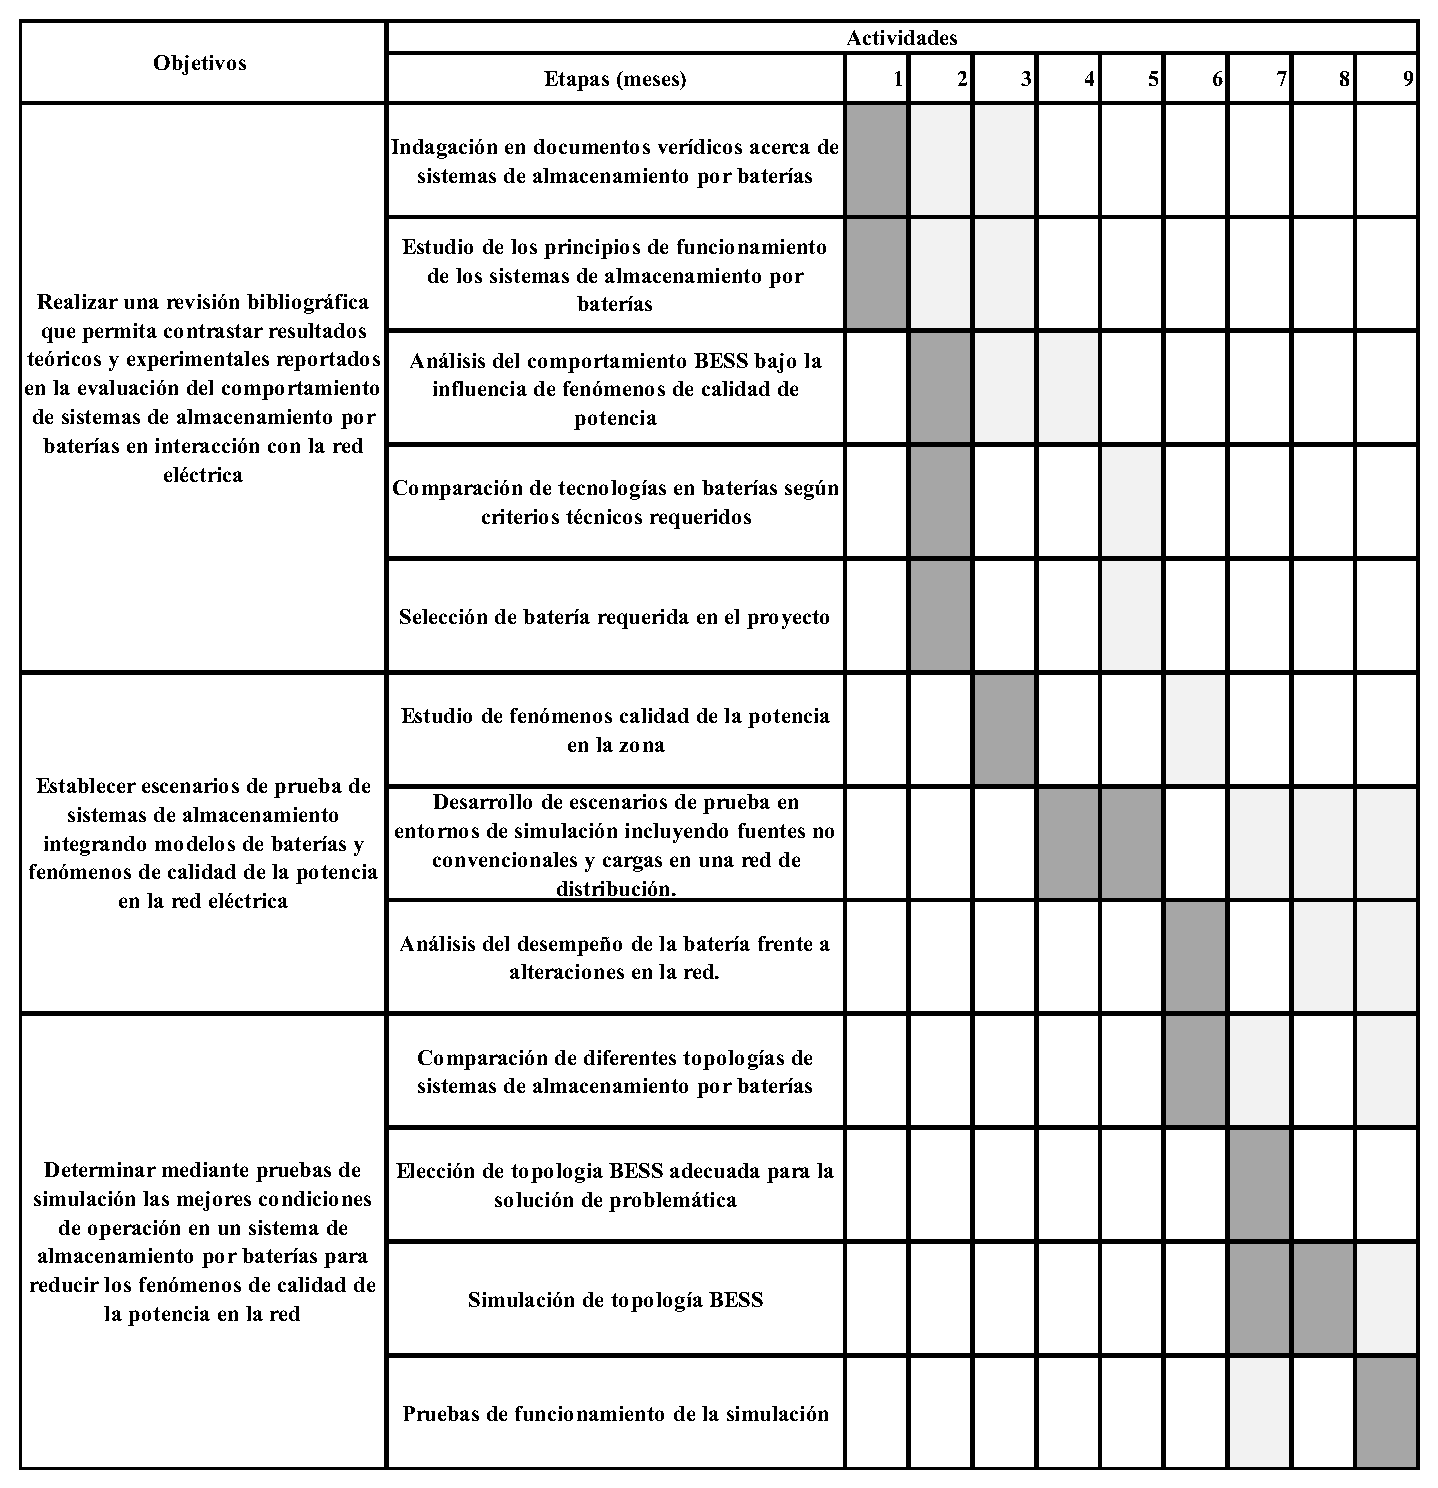
\includegraphics[scale=0.65]{Imágenes/cronograma/cronograma.eps}
	\caption{Cronograma}
    \end{center}
\end{table}


\newpage
\bibliographystyle{tesisUTP}
\phantomsection\addcontentsline{toc}{section}{\refname}
% Borrar linea \nocite{*} en el documento real.
% \nocite{*} imprime todas las referencias del archivo .bib, sin importar sin han sido referenciadas o no.  Por eso se debe borrar.
\nocite{*}
\bibliography{Referencias}
\end{document}
